\chapter{Einleitung}
\pagenumbering{arabic}
\section{Aufgabenstellung gemäss Eingabe}
Im Dokument 'Bachelorthesis-Aufgabe ist' folgendes festgehalten:
\begin{quote}
Seit mehreren Jahren bestreitet die HFTM unter der Leitung von Alain Rohr mit dem Solidus Team erfolgreich die internationalen Meisterschaften des RoboCups in der 'Logistics League'.
Das Team kennt sich meisterlich mit der Ansteuerung der Hardware aus, bittet aber die BFH um Mithilfe beim Software-Engineering.
Die Aufgabe dieser Arbeit ist es, ein Software-Design für die einzelnen Komponenten des verwendeten Roboters zu entwerfen. Angelehnt an die Vorgehensweise 'Domain Driven Design' soll konkret anhand des LIDARS gezeigt werden, wie das erarbeitete Software-Design implementiert und genutzt werden soll. Folgende Merkmale soll das Design mindestens aufweisen:

\begin{itemize}
	\item Die Schnittstelle der einzelnen Domänen muss Programmiersprachen-agnostisch sein
	\item Die Domänen müssen abgekapselt und unabhängig entwickelt und getestet werden können
	\item Das Design muss klar vorsehen, dass jedes Jahr das Entwicklungsteam komplett ausgetauscht wird
\end{itemize}
Bei dieser Arbeit gilt es auch zu beachten, dass die Software-Fähigkeiten des jeweiligen Entwicklungsteams erst noch ausgebildet werden müssen, es also nötig ist, die Schnittstellen so leicht und verständlich wie möglich zu halten, um nicht eine zu steile Lernkurve als Voraussetzung zu erschaffen.
\end{quote}
Im Kapitel \ref{sec:aufgabenstellung-messbar} wird die Messbare Aufgabenstellung (TODO) erläutert.

\section{HFTM Robocup}
\begin{figure}[H]
	\centering
	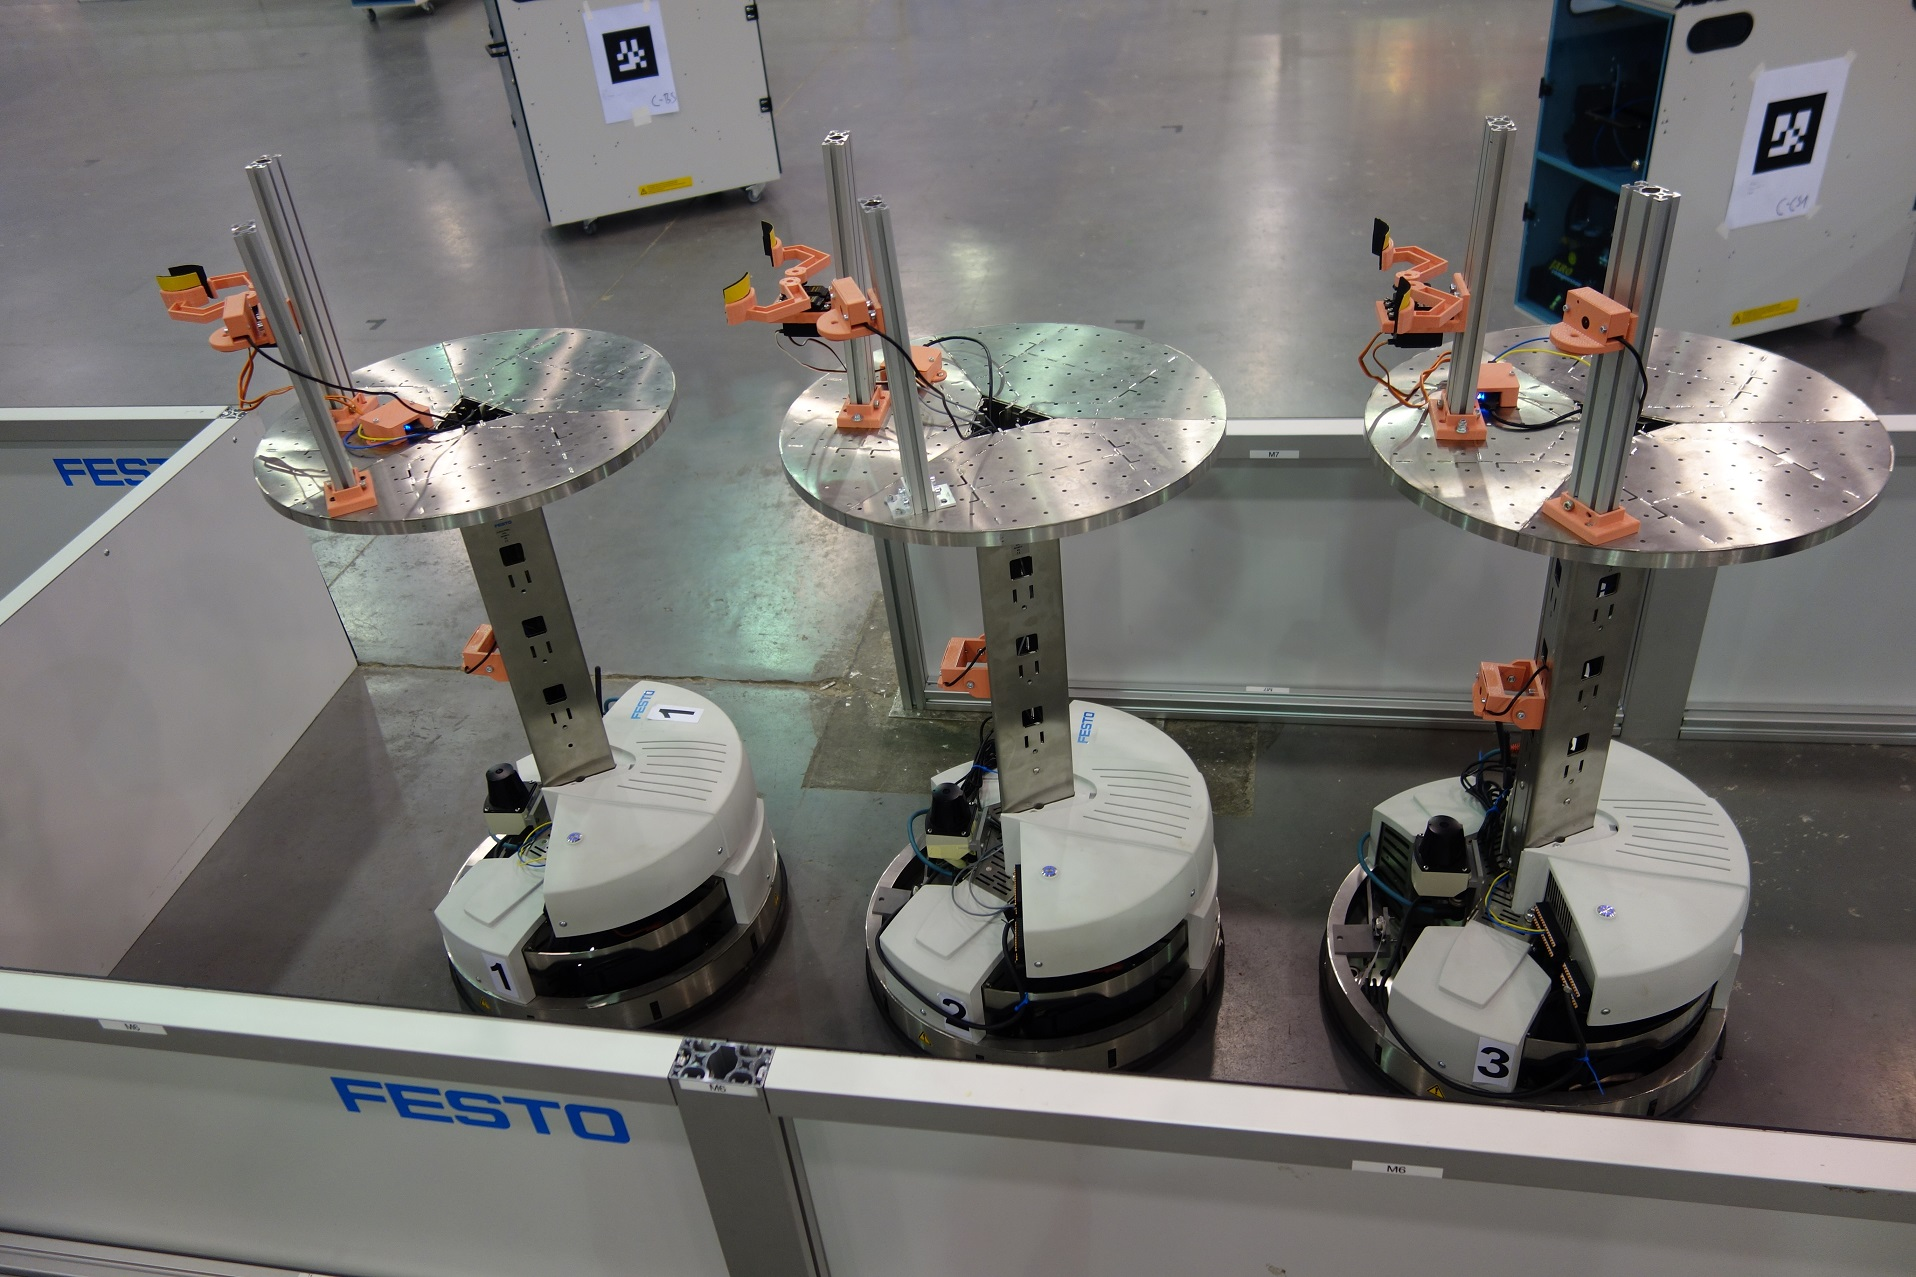
\includegraphics[width=0.5\textwidth]{img/robocup/robotino_v3.jpg}
	\caption{Robotino v3 für die Logistics League\cite{robotino}}
	\label{fig:robotino}
\end{figure}

TODO:
Roboter erklären, Schule erklären, Studienrichtung?

\section{Lidar}

\begin{figure}[H]
\centering
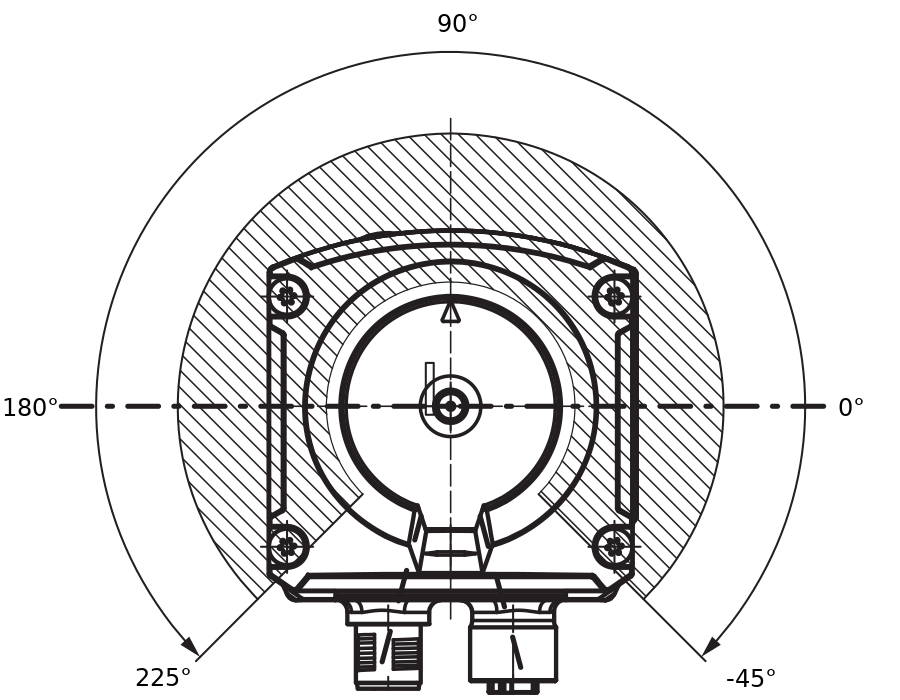
\includegraphics[width=0.5\textwidth]{img/lidar/lidar-coordinate.png}
\caption{\acrshort{lidar}-Koordinatensystem}
\label{fig:lidar}
\end{figure}

Beschreibung nach Datenblatt vom Hersteller Sick\cite{tim55x-techinfo}:
\begin{quote}
Der TiM5xx sendet mit einer Laserdiode gepulste Laserstrahlen aus. Trifft ein solcher Laserpuls auf ein Objekt oder eine Person, wird er an dessen Oberfläche reflektiert. Die Reflexion wird im Empfänger des TiM5xx von einer Fotodiode registriert. Der TiM5xx nutzt die SICK-eigene HDDM-Technologie (High Definition Distance Measurement). Bei diesem Messverfahren wird ein Messwert durch die Mittelwertbildung mehrerer Einzelpulse gebildet. Aus der Laufzeit, die das Licht von der Aussendung des Strahls bis zum Empfang der Reflexion benötigt, berechnet der TiM5xx die Entfernung zum Objekt. Dieses Prinzip der ,,Pulslaufzeitmessung'' wird in ähnlicher Form von Radarsystemen benutzt.

Mit einem rotierenden Spiegel lenkt der TiM5xx die ausgesendeten Laserstrahlen ab und tastet damit die Umgebung radial ab. Die Messungen werden intern von einem Winkelkodierer in regelmässigen Winkelschritten ausgelöst. Eine komplette Rotation stellt einen Messvorgang (Scan) dar. Der TiM5xx arbeitet mit einer Scanfrequenz von 15 Hz, d. h. er durchläuft 15 Messvorgänge pro Sekunde und stellt die Messergebnisse fortlaufend in Echtzeit über die Ethernet-Schnittstelle zur Verfügung.
\end{quote}

TODO:
was ist \acrshort{lidar}, wozu wird es verwendet, Funktionsweise High-Level





